\documentclass[french,12pt,a4paper]{article}
\usepackage[T1]{fontenc}
\usepackage[utf8]{inputenc}
\usepackage[dvips]{graphicx}
%\usepackage[english]{babel}
\usepackage[frenchb]{babel}
\AddThinSpaceBeforeFootnotes % à insérer si on utilise \usepackage[french]{babel}
\FrenchFootnotes % à insérer si on utilise \usepackage[french]{babel}
\usepackage{amsmath,amsthm,amsfonts,amssymb}
\usepackage{mathrsfs}
\usepackage{array}
\usepackage{color}
\usepackage{float}
\usepackage{pstricks,pstricks-add,pst-plot,pst-tree}
\usepackage{enumerate}
\usepackage{textcomp}
\usepackage{lscape}
\usepackage{setspace}
\usepackage{lettrine}
\usepackage{lscape}
\usepackage{lmodern}
\usepackage{stmaryrd}
\usepackage{subfigure}
\usepackage{multido}
\usepackage{listings}
\usepackage{footnote}
\usepackage{appendix}
\usepackage{color}
\usepackage{listings}
\usepackage{tikz}
\usepackage{dsfont}
\usetikzlibrary{matrix}

\lstset{
  language={C++},
  numbers=left, numberstyle=\tiny, stepnumber=1, firstnumber=last,
  frameround=tttt, 
  frame=single, 
  float,
  captionpos=b,
  breaklines=true,
  sensitive=f,
  morestring=[d]",
  basicstyle=\small\ttfamily,
  keywordstyle=\bf\small,
  stringstyle=\sf
}
\usepackage{fancyhdr,lastpage}
\usepackage[twoside,left=2cm,top=2.5cm,dvips,marginparwidth=1.9cm,marginparsep=0.5cm,headheight=35pt]{geometry}
%En tete et pied de page
\usepackage{fancyhdr}
\pagestyle{fancy}
\lhead{\leftmark} 
\chead{}
\rhead{PEPS}
\lfoot{ENSIMAG 3A}
\cfoot{\textit{Equipe 7}}
\rfoot{\thepage}
\renewcommand{\headrulewidth}{0pt}  
\renewcommand{\footrulewidth}{0.4pt}
\title{Projet .NET : Gestion indicielle}
\date{October 31, 475}
\author{Guillaume Fuchs, Guillaume Pelletier, Louis Perfumo, Samuel Rosilio}
%Page de garde

\begin{document}
\begin{titlepage}
\begin{center}

\textsc{\LARGE ENSIMAG}\\[1.5cm]

\textsc{\Large Projet d'évaluation de produit structuré}\\[0.5cm]

% Title
 \hrule
 \hrule 

\vspace{7mm}
{ \huge \bfseries Playlist 2  }

\vspace{7mm}
\hrule
\hrule

\vspace{7mm}
% Author and supervisor
\begin{minipage}{0.4\textwidth}
\begin{flushleft} \large
\emph{Etudiants:}\\
Guillaume \textsc{Fuchs},\\
Guillaume \textsc{Pelletier},\\
Samuel \textsc{Rosilio},\\
Louis \textsc{Perfumo}
\end{flushleft}
\end{minipage}

\vfill

% Bottom of the page
{\large \today}

\end{center}
\end{titlepage}
\tableofcontents
\newpage

\section{Introduction}

Ce rapport est l'objet d'une analyse du produit structuré nommé \lstinline!Playlist 2! déposé par  la CACEIS Bank, commercialisé par le réseau des caisses d'épargne et géré par Natixis Asset Management.
Ce produit est un OPCVM français qui pouvait être acheté entre le 14 janvier 2010 et le 28 juin 2010 avec pour valeur nominale liquidative de référence la valeur le maximale parmi toutes les valeurs liquidatives entre le 14 janvier et le 28 juin 2010. L'objectif de gestion du FCP est de permettre au porteur de recevoir la valeur liquidative de référence majorée d'un gain final à une date donnée dépendant des performances de 4 indices boursiers. 


\section{Définition}

Le \textbf{dépositaire} du produit financier est l'organisme qui sera chargé de :\\
\begin{itemize}
\item[•]
	La garde des avoirs en dépôt et leur restitution.
\item[•]
	Le dépouillement des ordres.
\item[•]
	L'information de la société de gestion ou de la SICAV des opérations relatives aux titres conservés pour son compte.
\item[•]
	Le contrôle de la régularité des décisions de l'OPC ou de sa société de gestion par rapport aux dispositions législatives et réglementaires applicables.\\
\end{itemize}


La \textbf{société de gestion} associée au produit devra s'occuper de :\\
\begin{itemize}
\item[•]
	La gestion de portefeuille pour le compte de tiers ce qui consiste à gérer des portefeuilles individuels d'instruments financiers pour le compte de clients, qu'il s'agisse par exemple de clients particuliers ou d'investisseurs institutionnels. Un mandat de gestion est conclu entre la société de gestion et son client.
\item[•]
	La gestion collective ou gestion d’organismes de placement collectif (OPC) consiste schématiquement à gérer des portefeuilles collectifs. Un OPC est constitué des sommes mises en commun par des investisseurs et gérées pour leur compte par un gestionnaire de portefeuille. Ce dernier utilise ces sommes pour acquérir des instruments financiers, par exemple des actions ou des obligations en fonction de ses objectifs. Des parts ou des actions représentant une quote-part de l’avoir de l’OPC sont émises, en contrepartie des sommes versées dans l’OPC. \\
\end{itemize}


Un FCP fait parti de la famille des OPCVM.\\
\begin{itemize}


\item[•]
Un \textbf{OPCVM} est une entité qui gère un portefeuille dont les fonds sont placés en valeurs mobilières. Garantie de l’investissement.\\

\item[•]
Une \textbf{OAT} est une obligation assimilable du Trésor, emprunts d’Etat émis pour une durée de 5 à 50 ans.\\

\item[•]
Un \textbf{fonds à formule} regroupe plusieurs catégories d’OPCVM. Il offre une perspective de gain dépendant des évolutions des marchés financiers, selon des paramètres définis à la souscription. Il offre une garantie sur le capital initialement investi. Il s'occupe de la gestion active du fonds dans des actifs non-risqués (monétaires, obligataires …) pour garantir le capital et des actifs risqués (actions, dérivées …) à la recherche de performance.\\

\item[•]
Une \textbf{OCDE} est une organisation de coopération et de développement économique. Elle publie des études statistiques. Les membres ont un système de gouvernement démocratique et une économie de marché.\\

\item[•]
Une \textbf{caisse d’amortissement de la dette sociale} est un organisme gouvernemental français qui possède de la dette sociale.\\

\item[•]
La \textbf{BPCE} est l'ensemble des entreprises qui composent la Caisse nationale des Caisses d’épargne et de la Banque fédérale des Banques populaires.\\

\item[•]
Le \textbf{dépositaire} d'un OPCVM est un établissement qui assure la conservation des actifs et le contrôle de la régularité des décisions de l'OPCVM.\\

\item[•]
La \textbf{société de gestion} d'un OPCVM est chargée de la gestion administrative, comptable et financière de l'OPCVM.\\

\item[•]
Le \textbf{FCP de capitalisation des revenus} représente tous les revenus investis dans le portefeuille du fonds propre.\\

\item[•]
Un \textbf{indice boursier} est une mesure statistique calculée par le regroupement des valeurs de titres de plusieurs sociétés.\\
Attention les indices des grands marchés mondiaux sont de plus en plus corrélés entre eux.\\

\item[•]
La \textbf{valeur liquidative} est la division de l’actif net de l’OPCVM par son nombre de parts calculée toutes les 2 semaines. Ceci implique des actifs d'une valeur inférieure à 80 millions €.\\

\item[•]
La \textbf{date de clôture de l'exercice} est la date à laquelle les résultats de l'année sont calculés.\\

\item[•]
La \textbf{performance} est la plus ou moins-value réalisée par rapport à l’investissement initial.\\

\item[•]
La \textbf{performance avec dividendes réinvestis} consiste en le fait que les dividendes sont réinvestis le jour même pour souscrire des actions supplémentaires. Cela permet d’estimer l’évolution véritable de la valeur de l’OPCVM, indépendamment de son mode de distribution. \\

\item[•]
Une \textbf{cession temporaire des titres} consiste en la vente de titres contre espèces ou autres titres avec un engagement irrévocable de part et d’autres de restituer les valeurs échangées.\\

\item[•]
Un \textbf{titre garanti} est un titre comportant un garant.\\

\item[•]
Un \textbf{Swap de performance} consiste à échanger de la performance d'une action contre un taux d'intérêt.\\

\item[•]
Une \textbf{exposition} (financière) est une limitation financière.\\

\item[•]
Un \textbf{Warrant} est un produit boursier à effet de levier qui donne le droit d'acheter ou de vendre à un prix donné un produit financier.\\

\item[•]
Un \textbf{Asset Swap} en terme général est un Swap sur actif.\\

\item[•]
Un \textbf{Swap} est un contrat d'échange de flux financiers entre deux parties jusqu'à une maturité et à fréquence déterminée.\\

\item[•]
Un \textbf{Cap} est un produit financier visant à assurer par son achat un niveau maximal sur un indice de taux révisable tout en profitant d'une éventuelle stabilité ou baisse de ce taux révisable. L'acheteur de Cap paie une prime au vendeur de Cap.\\

\item[•]
Un \textbf{Floor} est un produit financier visant à assurer par son achat un niveau minimal sur un indice de taux révisable tout en profitant d'une éventuelle stabilité ou hausse de ce taux révisable. L'acheteur d'un Floor paie une prime au vendeur du Floor.\\

\item[•]
Un \textbf{Collar} consiste en l'achat d'un Cap et la vente d'un Floor. L'objectif est de réduire le coût de la couverture contre le risque de taux.\\

\item[•]
Un \textbf{FRA} est un produit dérivé du marché monétaire. Il s'agit d'un contrat Forward, négocié sur le marché OTC (marché de gré à gré), entre deux contreparties et dont l'objectif est la fixation dès aujourd'hui d'un taux in fine de référence convenu sur un principal donné, pendant une période future spécifiée.\\

\item[•]
Les \textbf{titres de taux} regroupent l'ensemble des obligations à taux fixe et à taux variable. \\

\item[•]
Un \textbf{emprunt d'espèces} est un emprunt de liquidité sous forme de trésorerie. A comparer avec l'emprunt de titres.\\

\item[•]
Un \textbf{dépôt} est une opération de prêt qui génère une créance dans le patrimoine de l'OPCVM et une dette pour la banque. \\

\item[•]
La \textbf{prise et mise en pension} (cession de titre) est relative au taux REPO qui désigne une transaction dans laquelle deux parties s'entendent simultanément sur deux transactions: une vente de titres au comptant suivie d'un rachat à terme à une date et à un prix convenu d'avance. Cette transaction est qualifiée de pension livrée (prise en pension des titres par le prêteur de cash et mise en pension des titres par le prêteur de titres).\\

\item[•]
Le \textbf{titre de créance négociable} est un instrument financier qui suivant la nature de l'émetteur peut être: un Bon du Trésor à taux fixe (titre à court terme émis par le Trésor), un Bon du Trésor à intérêts annuels (titre moyen terme émis par le Trésor), un billet de trésorerie émis par les entreprises, un certificat de dépôts émis par les banques, un bon à moyen terme négociable émis par les entreprises et les établissements de crédit, un bon des institutions financières spécialisées émis par certains établissements du secteur financier public ou para-public.\\

\end{itemize}

\newpage
\section{Analyse des flux financiers du produit}

\subsection{Description du produit}

Notre produit financier prend appui sur l'évolution de 4 indices boursiers à travers le monde, les flux versés dépendront en effet des performances de chacun de ces indices depuis leur niveau d'origines (moyenne arithmétique des niveaux de clôture publiés le 29 avril 2010, 30 avril 2010 et le 3 mai 2010).
Les quatre indices considérés sont le Footsie 100, le Standard \& Poor's 500, Dow Jones Euro Stoxx 50 et le Nikkei 225.\\
\indent Le fonctionnement de notre produit est alors le suivant, si le 25 avril 2011 au moins trois des quatre indices ont eu un rendement supérieur à 10\%  alors un flux d'au moins 104,5\% de la valeur nominale nous sera versé à échéance. De plus si trois des quatre indices ont eu un rendement supérieur à 20\% alors la date d'échéance devient le 2 avril 2011 et nous recevons 104,5\% de la valeur nominale.\\
\indent En date du 23 avril 2012, nous raisonnons de la même façon en effet si trois des quatre indices ont eu un rendement supérieur à 10\% par rapport à leur niveau d'origine alors on obtiendra 4,5\% de plus que ce que l'on devrait déjà acquérir. En revanche si trois des quatre indices ont dépassé 20\% de rendement, la date d'échéance devient le 30 avril 2012.\\
Pour ce qui est des années 2013, 2014, 2015 et 2016, on accumule simplement 4,5\% en plus à échéance si trois des quatre indices ont un rendement supérieur à 10\% aux dates de constations. La date d'échéance finale (si aucun arrêt de la formule en 2011 et 2012) est le 25 avril 2016.\\

\subsection{Flux envisageables du produit}

\noindent Commençons par envisager les différents cas possibles :\\
Soit 
\[ A = \{ \text{Dow Jones Euro Stoxx 50}, \text{Standard \& Poor's 500}, \text{Footsie 100}, \text{Nikkei 225} \} \]\\
Ainsi 
\[ \forall \text{i, j, k, l} \in \text{A tels que A} = \{ \text{i, j, k, l} \} \]\\

\begin{itemize}

\item[•]
Cas où l'échéance est en fin de première année :\\

\begin{spacing}{1.2}
\begin{center}
\begin{tabular}{|c|c|c|c|c|c|}
  \hline
  Date & $R_{i}$ & $R_{j}$ & $R_{k}$ & $R_{l}$ & Prime accumulée \\
  \hline
  25/04/2011 & 21\% & 15.6\% & 22.6\% & 31.1\% & 4.5\%\\
  \hline
\end{tabular}
\end{center}
\end{spacing}
\indent \\
\indent \\
On constate dès la première année que trois des quatre indices dépassent un rendement de 20\% ainsi le produit arrive à échéance en fin de première année et le client recevra 104,5\% puisque par conséquent trois des quatre indices ont eu une performance supérieure à 10\% \\

\item[•]
Cas le moins intéressant pour le client avec échéance deux ans :\\

\begin{spacing}{1.2}
\begin{center}
\begin{tabular}{|c|c|c|c|c|c|}
  \hline
  Date & $R_{i}$ & $R_{j}$ & $R_{k}$ & $R_{l}$ & Prime accumulée \\
  \hline
  25/04/2011 & 5.8\% & 15.6\% & 2.6\% & -7.1\% & 0\%\\
  23/04/2012 & 21.3\% & 28.8\% & 20.4\% & 10.3\% & 4.5\%\\
  \hline
\end{tabular}
\end{center}
\end{spacing}
\indent \\
\indent \\
Dans ce cas ci, aucune prime n'est acquise grâce aux performances des indices la première année, de plus la seconde année comme trois des quatre performances dépassent 20\%, l'échéance devient le 30/04/2012 et 104,5\% sera versé au client.\\

\item[•]
Cas le plus intéressant pour le client avec échéance deux ans :\\
\begin{spacing}{1.2}
\begin{center}
\begin{tabular}{|c|c|c|c|c|c|}
  \hline
  Date & $R_{i}$ & $R_{j}$ & $R_{k}$ & $R_{l}$ & Prime accumulée \\
  \hline
  25/04/2011 & 13.8\% & 15.6\% & 10.6\% & -7.1\% & 4.5\% \\
  23/04/2012 & 21.3\% & 28.8\% & 20.4\% & 5.3\% & 9\% \\
  \hline
\end{tabular}
\end{center}
\end{spacing}
\indent \\
\indent \\
Ainsi dans ce cas le client recevra une prime de 9\% de la valeur liquidative de référence en fin de deuxième année. L'échéance devient donc le 30/04/2012 et 109\% de la valeur liquidative de référence sera versé au client.\\

\item[•]
Nous allons maintenant distinguer les deux cas extrêmes dans le cas d'une échéance à six ans, le premier cas correspond à celui où le client ne gagnera rien soit :\\
\begin{spacing}{1.2}
\begin{center}
\begin{tabular}{|c|c|c|c|c|c|}
  \hline
  Date & $R_{i}$ & $R_{j}$ & $R_{k}$ & $R_{l}$ & Prime accumulée \\
  \hline
  25/04/2011 & 3.8\% & 5.6\% & 0.6\% & -7.1\% & 0\% \\
  23/04/2012 & 10.3\% & 8.8\% & -10.4\% & 5.3\% & 0\% \\
  29/04/2013 & 4.5\% & 12.4\% & 4.2\% & 14.2\% & 0\%\\
  29/04/2014 & -5.4\% & 16.3\% & 10.2\% & 9.4\% & 0\%\\
  29/04/2015 & 3.3\% & 11.1\% & 7.1\% & 18.2\% & 0\%\\
  25/04/2016 & 11.5\% & 15.2\% & 8.7\% & 9.9\% & 0\%\\
  \hline
\end{tabular}
\end{center}
\end{spacing}
\indent \\
\indent \\
Dans ce cas ci qui est le cas le plus défavorable sur un horizon de six ans, le client retouchera la valeur liquidative de référence à la fin de la sixième année car trois des quatre indices n'ont jamais eu une performance supérieure à 10\%.\\

\newpage
\item[•]
Cas le plus favorable pour une échéance de six ans :\\
\begin{spacing}{1.2}
\begin{center}
\begin{tabular}{|c|c|c|c|c|c|}
  \hline
  Date & $R_{i}$ & $R_{j}$ & $R_{k}$ & $R_{l}$ & Prime accumulée \\
  \hline
  25/04/2011 & 13.8\% & 15.6\% & 10.6\% & -7.1\% & 4.5\% \\
  23/04/2012 & 10.3\% & 18.8\% & -10.4\% & 15.3\% & 9\% \\
  29/04/2013 & 14.5\% & 12.4\% & 4.2\% & 14.2\% & 13.5\%\\
  29/04/2014 & -5.4\% & 16.3\% & 10.2\% & 19.4\% & 18\%\\
  29/04/2015 & 3.3\% & 11.1\% & 17.1\% & 18.2\% & 22.5\%\\
  25/04/2016 & 21.5\% & 15.2\% & 18.7\% & 29.9\% & 27\%\\
  \hline
\end{tabular}
\end{center}
\end{spacing}
\indent \\
\indent \\
Dans ce cas ci, le client touchera à la fin de la sixième année 127\% de la valeur liquidative de référence puisque chaque année, au moins trois des quatre indices ont une performance supérieure à 10\%.\\
\end{itemize}

\noindent On peut résumer avec l'arbre suivant les flux possibles à échéance du produit (en notant 0 les nœuds non terminaux)  :

% Set the overall layout of the tree
\tikzstyle{level 1}=[level distance=4cm, sibling distance=3cm,->]
\tikzstyle{level 2}=[level distance=4cm, sibling distance=2cm,->]

% Define styles for bags and leafs
\tikzstyle{bag} = [text width=2em, text centered]
\tikzstyle{end} = []

% The sloped option gives rotated edge labels. Personally
% I find sloped labels a bit difficult to read. Remove the sloped options
% to get horizontal labels. 
\begin{tikzpicture}[>=stealth,sloped]
    \matrix (tree) [%
      matrix of nodes,
      minimum size=1cm,
      column sep=3cm,
      row sep=0.9cm,
    ]
    {
          &       &      & 190.5\\
          &       & 163.5  & 183.75\\
          & 156.75 &      & 177 \\
      150 &       & 156.75& 170.25 \\
          & 0   &      & 163.5 \\
          &       & 0  & 156.75\\
          &       &      & 150 \\
    };
    \draw[->] (tree-4-1) -- (tree-3-2) node [midway,above] {};
    \draw[->] (tree-4-1) -- (tree-5-2) node [midway,below] {};
    \draw[->] (tree-3-2) -- (tree-2-3) node [midway,above] {};
    \draw[->] (tree-3-2) -- (tree-4-3) node [midway,below] {};
    \draw[->] (tree-5-2) -- (tree-4-3) node [midway,above] {};
    \draw[->] (tree-5-2) -- (tree-6-3) node [midway,below] {};
    \draw[->] (tree-2-3) -- (tree-1-4) node [midway,below] {};
    \draw[->] (tree-2-3) -- (tree-2-4) node [midway,below] {};
    \draw[->] (tree-2-3) -- (tree-3-4) node [midway,below] {};
    \draw[->] (tree-2-3) -- (tree-4-4) node [midway,below] {};
    \draw[->] (tree-2-3) -- (tree-5-4) node [midway,below] {};
    \draw[->] (tree-4-3) -- (tree-2-4) node [midway,below] {};
    \draw[->] (tree-4-3) -- (tree-3-4) node [midway,below] {};
    \draw[->] (tree-4-3) -- (tree-4-4) node [midway,below] {};
    \draw[->] (tree-4-3) -- (tree-5-4) node [midway,below] {};
    \draw[->] (tree-4-3) -- (tree-6-4) node [midway,below] {};
    \draw[->] (tree-6-3) -- (tree-3-4) node [midway,below] {};
    \draw[->] (tree-6-3) -- (tree-4-4) node [midway,below] {};
    \draw[->] (tree-6-3) -- (tree-5-4) node [midway,below] {};
    \draw[->] (tree-6-3) -- (tree-6-4) node [midway,below] {};
    \draw[->] (tree-6-3) -- (tree-7-4) node [midway,below] {};
  \end{tikzpicture}



  \subsection{Rentabilités espérées du produit}

\noindent On peut avoir de même un tableau résumant les rentabilités actuarielles annuelles sous la forme suivante en considérant que le prix de départ est de la valeur liquidative de référence ( les x sont des cas impossibles) :

   \begin{tikzpicture}[>=stealth,sloped]
    \matrix (tree) [%
      matrix of nodes,
      minimum size=1cm,
      column sep=3cm,
      row sep=1cm,
    ]
    {
          &       &      & 4.06\%\\
          &       & 4.40\%  & 3.44\%\\
          & 4.50\% &      & 2.80\% \\
        0 &       & 2.23\% & 2.13\% \\
          & x   &      & 1.45\% \\
          &       & x  & 0.74\%\\
          &       &      & 0\% \\
    };
    \draw[->] (tree-4-1) -- (tree-3-2) node [midway,above] {};
    \draw[->] (tree-4-1) -- (tree-5-2) node [midway,below] {};
    \draw[->] (tree-3-2) -- (tree-2-3) node [midway,above] {};
    \draw[->] (tree-3-2) -- (tree-4-3) node [midway,below] {};
    \draw[->] (tree-5-2) -- (tree-4-3) node [midway,above] {};
    \draw[->] (tree-5-2) -- (tree-6-3) node [midway,below] {};
    \draw[->] (tree-2-3) -- (tree-1-4) node [midway,below] {};
    \draw[->] (tree-2-3) -- (tree-2-4) node [midway,below] {};
    \draw[->] (tree-2-3) -- (tree-3-4) node [midway,below] {};
    \draw[->] (tree-2-3) -- (tree-4-4) node [midway,below] {};
    \draw[->] (tree-2-3) -- (tree-5-4) node [midway,below] {};
    \draw[->] (tree-4-3) -- (tree-2-4) node [midway,below] {};
    \draw[->] (tree-4-3) -- (tree-3-4) node [midway,below] {};
    \draw[->] (tree-4-3) -- (tree-4-4) node [midway,below] {};
    \draw[->] (tree-4-3) -- (tree-5-4) node [midway,below] {};
    \draw[->] (tree-4-3) -- (tree-6-4) node [midway,below] {};
    \draw[->] (tree-6-3) -- (tree-3-4) node [midway,below] {};
    \draw[->] (tree-6-3) -- (tree-4-4) node [midway,below] {};
    \draw[->] (tree-6-3) -- (tree-5-4) node [midway,below] {};
    \draw[->] (tree-6-3) -- (tree-6-4) node [midway,below] {};
    \draw[->] (tree-6-3) -- (tree-7-4) node [midway,below] {};
  \end{tikzpicture}

  \subsection{Expression analytique des flux}
\noindent Soit 
\[ A = \{ \text{Dow Jones Euro Stoxx 50}, \text{Standard \& Poor's 500}, \text{Footsie 100}, \text{Nikkei 225} \} \]\\

\noindent et

\[ B = \{1,2,6\} \]\\
\\
\\
On cherche alors à déterminer le flux qui sera versé à la date t en fonction de la valeur liquidative de référence notée $N_{0}$.
On obtient alors pour $t \in \left\lbrace 1,2,3,4,5,6 \right\rbrace$ :

\begin{multline*}

  F_{versé}(t) = N_{0}*(1+ \sum_{i=1}^{t}(4.5\%*\mathds{1}_{\left\lbrace \sum_{I \in A} \mathds{1}_{\left\lbrace Perf_{I}(i)>10\% \right\rbrace}>2 \right\rbrace}) * (\mathds{1}_{\left\lbrace \sum_{I \in A} \mathds{1}_{\left\lbrace Perf_{I}(\min{(t,2)})>20\% \right\rbrace}>2 \right\rbrace}\\ 
  + \mathds{1}_{\mathds{1}_{t=6}}*\mathds{1}_{\left\lbrace \sum_{I \in A} \mathds{1}_{\left\lbrace Perf_{I}(1)>20\% \right\rbrace}<3 \right\rbrace}*\mathds{1}_{\left\lbrace \sum_{I \in A} \mathds{1}_{\left\lbrace Perf_{I}(2)>20\% \right\rbrace}<3 \right\rbrace})*\mathds{1}_{\{t \in B\}}) \\
  
\end{multline*}

Analysons cette formule, dans un premier temps $\mathds{1}_{\{t \in B\}}$ représente le fait que des flux ne peuvent être versés que si nous sommes en $t=1$ ou 2 ou 6. De plus, $\mathds{1}_{\mathds{1}_{t=6}}*\mathds{1}_{\left\lbrace \sum_{I \in A} \mathds{1}_{\left\lbrace Perf_{I}(1)>20\% \right\rbrace}<3 \right\rbrace}*\mathds{1}_{\left\lbrace \sum_{I \in A} \mathds{1}_{\left\lbrace Perf_{I}(2)>20\% \right\rbrace}<3 \right\rbrace}$ représente le fait que en $t=6$ un flux ne peut être versé que si moins de trois indices ont eu une performance inférieure à 20\% en $t=1$ et en $t=2$. Le terme $\mathds{1}_{\left\lbrace \sum_{I \in A} \mathds{1}_{\left\lbrace Perf_{I}(\min{(t,2)})>20\% \right\rbrace}>2 \right\rbrace}$ permet quant à lui de détecter le fait qu'un flux est versé en $t=1$ ou $t=2$. Enfin le terme du début permet simplement de calculer le flux versé. 

\section{Clients visés}

Afin de mieux comprendre les risques et le produit, nous devons réfléchir aux types d'investisseurs concernés par un tel produit.\\

\indent \textbf{Le Montant minimum à la première souscription} est de 150 euros. Ce montant est faible comparé au montant minimum de souscription dans le cas d'obligations qui est généralement de l'ordre de quelques milliers d'euros, ou encore pour se créer un portefeuille d'actions diversifié. En effet, certaines actions peuvent atteindre plusieurs centaines d'euros l'unité. Ce montant de 150 euros pour une souscription permet à un particulier d'investir dans cet OPCVM.\\
\indent Les simulations sur les données historique de marché permettent de calculer des rendements fictifs, calculés en fonction des dates d'échéance passées de la formule. Elles permettent de visualiser le comportement de la formule lors des différentes phases de marché traversées au moments de simulations.\\

\begin{center}
\caption{Simulations sur des données historiques de marché}
\end{center}

\begin{center}
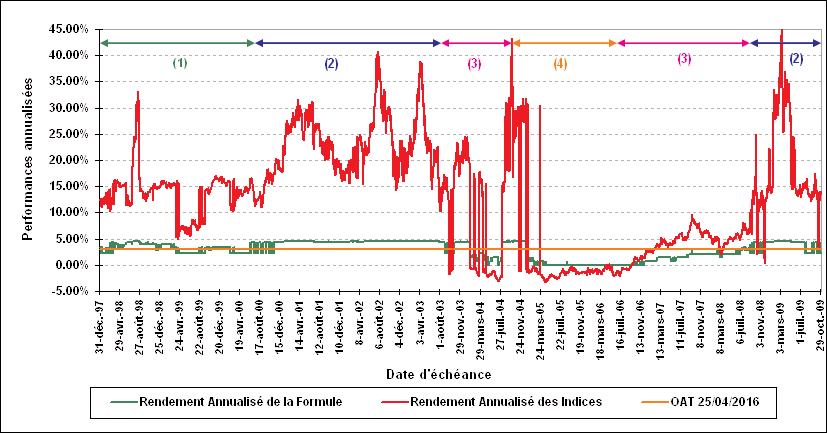
\includegraphics[scale=0.5]{simulations_historiques.png}
\end{center}

\indent Sur les simulations réalisées entre le 31 décembre 1991 et le 3 novembre 2009 on remarque que le rendement du FCP reste positif ou nul (hors commission de souscription) quelles que soit les phases de marché traversées. Néanmoins on remarque que le rendement des indices lors de hausse des marchés est très élevé par rapport au rendement de de la formule qui est en moyenne supérieur au taux sans risque. Lors de phase de volatilité des marchés, alors que les performances des indices n'obéissent pas à une tendance claire, le rendement du FCP reste positif ou nul et est supérieur au taux sans risque. Enfin pendant une période de chute des marchés, tandis que les indices ont des performances négatives, le rendement du FCP reste positif ou nul mais inférieur au taux sans risque. \\
\indent Ces simulations de scénarios montrent donc que la formule permet un rendement équivalent à un taux sans risque bien qu'il arrive lors de chute des marchés que le rendement du FCP soit nul. Lors de situation de marché stable où les indices sont élevés, les performances de la formule est nettement inférieur aux performances des indices. \\
\indent L'OPCVM permet donc à un particulier d'investir dans un actif comparable à un taux sans risque. Il permet en plus d'avoir un produit qui suit les performances des indices sur des dates d'échéances. Néanmoins le produit n'est pas comparable à un Tracker car globalement la formule n'engendre pas des rendements du même ordre de grandeur que les indices. Les institutions financières qui cherche à investir dans des actifs peu risqués utiliseront plutôt des obligations tandis que s'il cherchent à obtenir un rendement élevés qui suivent les performances des 4 indices, ils achèteront des Tracker. De plus le Fonds est plafonné à 924 459 parts, de valeur nominale de 150€, ce qui fait un total de 138 668 850€. Ce montant est faible pour des investisseurs qui seraient des institutions financières.\\
\indent L'OPCVM se veut donc un produit pour des particuliers qui souhaitent obtenir un rendement similaire au taux sans risque avec une prise de risque faible. L'OPCVM garantit ainsi un rendement positif ou nul quelles que soient les fluctuations du marché. De plus un placement en OPCVM permet d'obtenir un portefeuille diversifié tout en restant accessible par son prix de souscription minimum faible et sécurisé grâce au cadre légal et réglementaire.\\

\newpage
\section{Analyse des risques du produit}

Dans cette partie, nous allons analyser tous les points qui peuvent constituer un risque pour la banque émettrice du produit puis pour le détenteur du produit. \\


\subsection{Risques pour la Banque}


\indent La banque est exposée au \textbf{risque de couverture}. La banque va devoir être en mesure de payer au porteur à l'une des dates d'échéances anticipées ou à la date d'échéance maximum, la valeur liquidative de référence, hors commission de souscription, majorée d'un gain final qui est acquis au cours du temps. Une fluctuation des marchés durant la durée de vie de la formule peut rendre moins efficace la couverture mise en place par la société de gestion. Le risque de couverture peut se matérialiser sous la forme d'autres risques: le risque de contrepartie, le risque sur la volatilité, risque de liquidité et le risque de taux. \\

\indent \textbf{Le risque de contrepartie} est le risque que ses clients soient dans l'incapacité de rembourser leurs emprunts, ou qu'une institution financière avec laquelle le fonds a des opérations en cours soit défaillante. Ce risque est présent car le portefeuille de l'OPCVM est constitué d'actifs qui entrent dans ces deux catégories.\\
\indent Pour illustrer ce risque, prenons un Swap de taux payeur (le taux fixe est payé, et le taux variable est perçu), conclu avec une contrepartie qui se finance intégralement à taux variable. Lorsque les taux augmentent, la rentabilité et donc la valeur de ce Swap de taux payeur augmente, cependant la qualité de crédit de la contrepartie qui se finance à taux variable baisse puisque le coût de son financement a augmenté. Dans cet exemple, le Swap de taux payeur est soumis au risque que l'exposition à la contrepartie soit inversement corrélée à la qualité de crédit de celle-ci. \\
\indent Une manière de se couvrir contre ce risque de contrepartie consiste à diversifier les Swaps avec différentes institutions financières. Plus les Swaps sont établis avec un nombre d'institutions financières différentes et plus les pertes engendrées par les Swaps sont réduites.\\
Une autre manière consiste à établir des CDS avec d'autres contreparties. Lors de la défaillance d'une contrepartie sur un Swap, le contrat permettra de se protéger contre la perte possible par le biais du vendeur de CDS qui se porte garant. Pour ce faire, la personne désireuse de se protéger (ici la société de gestion) contre une défaillance de contrepartie (ici la contrepartie du Swap) paie à un tiers un flux régulier et reçoit de ce tiers un paiement défini à l'origine en cas de survenance de la défaillance redoutée. Selon l'ISDA (International Swaps and Derivates Association), les évènements de crédits concernent dans notre cas les défauts de paiements de la contrepartie du Swap.\\

\indent L'objectif de gestion du FCP est de permettre aux porteurs de recevoir aux dates d'échéances anticipées ou à la date d'échéance finale la valeur liquidative de référence avec le gain engendré durant la période. Si le portefeuille d'OPCVM est constitué d'actifs risqués alors \textbf{le risque de volatilité} augmenterait l'incertitude des rendements qu'engendrent les actifs et donc le rendement final garanti aux porteurs. \\
\indent C'est par exemple le cas de l'action d'une société plus endettée, ou disposant d'un potentiel de croissance plus fort et donc d'un cours plus élevé que la moyenne. Si la croissance des ventes est moins forte qu'espérée ou si l'entreprise peine à rembourser sa dette, la chute du cours sera très forte. \\
\indent Il est possible de tirer parti d'une volatilité élevée. Par exemple, prendre une position longue sur la volatilité peut être intéressant sur le plan tactique: la propension naturelle au retour vers la moyenne de la volatilité implicite offre des opportunités d'achat de couverture lorsque la volatilité retourne vers la moyenne après s'être hissée à un niveau élevé. \\
Les couvertures possibles se font grâce à des actifs financiers qui limitent l'achat maximale ou la vente minimale d'un actif. Des options exotiques comme les options Lookback permettent d'engendrer un gain important lorsque les marchés deviennent très volatiles. Les options Barrières permettent de limiter la prime payée sur ces options grâce à une volatilité élevée qui va enclencher la barrière et activer l'option. Les FRA, les Caps, les Floors et les Swaps vont permettre à la société de gestion de limiter le taux maximale pour l'emprunt (achat d'un FRA, Cap ou Swap payeur) ou limiter le taux minimale pour le prêt (achat d'un Floor). \\


\indent \textbf{Le risque de liquidité} implique qu'une position, dans le portefeuille de l'OPCVM, ne puisse être cédée, liquidée ou clôturée pour un coût limité et dans un délai suffisamment court, compromettant ainsi la capacité de l'OPCVM à se conformer aux dates d'échéances et aux dispositions qui sont prévus pour le client. Si les marchés sont peu liquides, l'efficacité de la couverture est diminuée car la banque rencontrera des difficultés à acheter ou vendre les actifs de couverture aux moments nécessaires. \\
\indent Par exemple, financer des crédits 10 ans par des emprunts à 3 mois représente un risque majeur en termes de liquidité. En effet, tous les trois mois, il faut trouver le refinancement et cela pendant 10 ans. En revanche, à l'inverse si on finance des crédits 5 ans par des emprunts 10 ans le risque de liquidité est minime. Pour se fixer des limites en liquidité, il faut donc se fixer un niveau de transformation sur chaque maturité. \\
\indent Le Cash at Risk est une mesure du risque de liquidité. Elle se mesure soit à partir de la comparaison des échéances contractuelles des dettes et des estimations des recettes de trésorerie, ou bien à travers un budget de trésorerie. Cet indicateur reprend globalement les modélisations issues des calculs de Value at Risk. Le calcul de cette mesure avant d'investir dans un actif va permettre de savoir l'exposition au risque de liquidité que prend l'institution. Cette mesure permet aussi d'obtenir des informations sur le risque de liquidité d'actifs déjà en possession. Une augmentation du Cash at Risk d'un produit peut permettre de liquider une position avant que la vente soit impossible. 
\\

\indent La variation des taux d'intérêts a un impact sur la variation du prix ou la valorisation d'un actif. La société de gestion possède donc un \textbf{risque de taux} sur l'ensemble de ses actifs. L'évolution des taux d'intérêts va générer un effet inverse sur le cours des obligations. \\
\indent Par exemple, le risque de taux se matérialise quand une banque refinançant un prêt à long terme à taux fixe par un emprunt à taux variable fait face à une hausse brutale des taux d'intérêts. Le risque est d'autant plus élevé que la maturité des actifs à taux fixe est éloignée et que la proportion d'actifs à taux fixe est importante dans le bilan de l'OPCVM.\\
\indent Pour se couvrir, on détermine par maturité la sensibilité du portefeuille au taux. On réduit cette sensibilité si on anticipe une hausse des taux et on augmente cette sensibilité si on anticipe une baisse. Plusieurs contrats permettent de se couvrir contre ce risque: les Swaps, les Caps ou les Collars.\\

\indent Pour un OPCVM de la zone euro, le \textbf{risque de change}, c'est-à-dire la variation des cours d'une devise -autre que l'euro - dans laquelle un fonds aurait investi, est présent. Le risque de change tient au fait que l'intérêt sur les obligations puis le remboursement du capital peut être payé dans une devise faible, ou qui se dévalue, et par conséquent le paiement des intérêts et le rendement final de l'investissement sera donc plus faible que celui attendu par l'investisseur et idem pour le capital.\\
\indent Playlist 2 est un OPCVM libellé en euros jouant sur les marchés internationaux et n'est pas donc pas exempt de ce risque. En effet la devise principale de l'investisseur est l'euro. Le portefeuille de l'OPCVM est donc valorisé en euro, néanmoins la devise des obligations dans lequel l'OPCVM investit peut être dans une monnaie différente comme le dollar qui peut aussi bien s'apprécier que se déprécier face à la monnaie européenne. \\
\indent Pour se couvrir contre le risque de change, on détermine une position par devise. On gère cette position en la couvrant via des actifs financiers comme des Swaps, des Caps ou des FRA sur taux ou encore des options Quanto en euro(similaire à une option classique sur un actif étranger où les flux récupéré lors de l'activation de l'option sont en euro) qui vont permettre de limiter ce risque de change. \\

\indent Un OPCVM possède une exposition au \textbf{risque d'actions}. Elle tient compte des opérations en cours et notamment de celles réalisées sur les marchés des dérivés, qui peuvent augmenter ou diminuer les risques de la gestion selon les fluctuations des marchés et du prix de l'action. \\
Avoir un seuil d'exposition minimum au risque d'actions de 60\% signifie que les gérants ne pourront à aucun moment réduire l'exposition en-deçà de ce seuil, de façon à maintenir une corrélation étroite avec l'évolution des marchés conforme à la nature de cette catégorie d'OPCVM.\\
Une couverture sur le risque d'action peut se faire par le biais de contrats d'achat ou de vente passés à l'avance grâce à des produits dérivés fermes (Futures ou Forwards) ou des produits dérivés optionnels (options).\\


\subsection{Risques pour le détenteur}

\indent En souscrivant au fonds, le détenteur, s'il garde ses parts, est assuré de récupérer au moins la Valeur Liquidative de Référence majorée du gain final. Cependant, cette valeur peut être sensibles à de nombreux risques présents sur les marchés et auxquels la banque doit se couvrir comme expliqué plus haut. Le détenteur n'est donc pas à l'abri de voir la valeur de son investissement diminuer au cours de sa participation dans la formule.\\

\indent Le détenteur du produit est exposé au risque financier systémique sur les 4 marchés de référence pour l'OPCVM. Une absence d'augmentation de la performance d'au moins 10\% des indices aux dates de constatations entraînera un gain final réduit.\\
Le porteur ne peut se couvrir contre cette absence d'augmentation des marchés.\\

\indent Le détenteur est exposé au risque que le fonds soit dissous ou soit fusionné. Dans ce cas, les détenteurs de parts pourraient voir sa valeur liquidative garanti réduite. En effet, en souscrivant à l'OPCVM, le porteur peut choisir qu'en cas de liquidation du fonds il est remboursé par la société garante en numéraire ou en titres. Dans le cas des titres, le risque que les titres reçus ne soient pas liquides sont grands car dans le cas d'une liquidation du fonds, la société de gestion n'a pas pu vendre ses actifs. Dans le cas du numéraire, le risque pour le porteur est que le garant ne possède pas assez de trésorerie pour rembourser tous les épargnants. \\
Pour se couvrir contre un tel risque, une étude de la répartition des remboursements est à voir. Généralement, investir beaucoup dans un OPCVM permet d'avoir une priorité sur le remboursement en cas de liquidation. \\

\indent Le client est également exposé à risque d'augmentation de l'inflation en effet malgré de potentielle gain il peut voir son pouvoir d'achat diminuer. \\
\indent En cas d'augmentation de l'inflation, lors du versement des liquidités par le FCP, les revenus perçus seront déprécié au cours du temps. La valeur liquidative de référence n'est donc pas exactement celle à laquelle le porteur aurait pu s'attendre.\\
\indent Une couverture contre l'inflation est par le biais d'un intermédiaire bancaire d'investir dans des produits indexés sur l'inflation. Les OAT et les Swaps d'inflation française permettent de se couvrir contre ce risque.\\



\subsection{Synthèse des risques}

\noindent Les risques énoncés précédemment peuvent donc être synthétisés selon le tableau suivant :\\

\begin{spacing}{1.2}
\begin{center}
\begin{tabular}{|c|c|c|}
  \hline
  Type de risque & Détenteur & Banque \\
  \hline
  Risque de valeur de la VLR & \checkmark &  \\
  \hline
  Risque de contrepartie & \checkmark &  \\
  \hline
  Risque de marché & \checkmark & \checkmark\\
  \hline
  Risque de couverture &  & \checkmark \\
  \hline
  Risque de volatilité &  & \checkmark \\
  \hline
  Risque de liquidité &  & \checkmark\\
  \hline
  Risque d'inflation & \checkmark & \\
  \hline 
  Risque de change &  & \checkmark \\
  \hline
  Risque d'actions &  & \checkmark\\
  \hline
  Risque de taux &  & \checkmark\\
  \hline
\end{tabular}
\end{center}
\end{spacing}
 

\section{Corrélation entre les indices}

Nous avons cherché à déterminer dans cette partie si il existait des corrélations entre les performances des différents indices en présence auquel cas, à partir de l'évolution d'un des indice on pourrait selon un certain intervalle de confiance prévoir l'évolution de la performance de certains autres indices parmi les 4 indices.  
C'est ainsi que nous avons commencé par calculer les différentes performances de chaque indice depuis le 29 avril 2010, puis que nous avons utilisé le logiciel R pour déterminer ces corrélations. 

\begin{spacing}{1.2}
\begin{center}
\begin{tabular}{|c|c|c|c|c|}
  \hline
   & Footsie 100 & Eurostoxx 50 & Nikkei 225 & S\& P 500 \\
  \hline
  Footsie 100 & 1 & 0.568 & 0.848 & 0.894\\
  Eurostoxx 50 & 0.568 & 1 & 0.507 & 0.278 \\
  Nikkei 225 & 0.848 & 0.507 & 1 & 0.822\\
  S \& P 500 & 0.894 & 0.278 & 0.822 & 1\\
  \hline
\end{tabular}
\end{center}
\end{spacing}

Afin d'observer au mieux les corrélations relevées ci dessus, nous avons décidé de tracer les performances de chaque indice jour par jour en prenant comme point de référence les valeurs des cours le 29/04/2010 et le 30/04/2010 pour le Nikkei 225 puisque celui ci n'était pas côté le 29/04/2010.
Aux vues des corrélations obtenues précédemment, nous devrions observé des rentabilités évoluant la plupart du temps dans le même sens et les mêmes proportions pour les couples (Footsie,Nikkei), (Footsie,S \& P) et finalement de manière un peu moindre entre (Nikkei, S \& P).


\begin{center}
\caption{Performances des différents indices du produit depuis le 29/10/2010}
\end{center}


\begin{center}
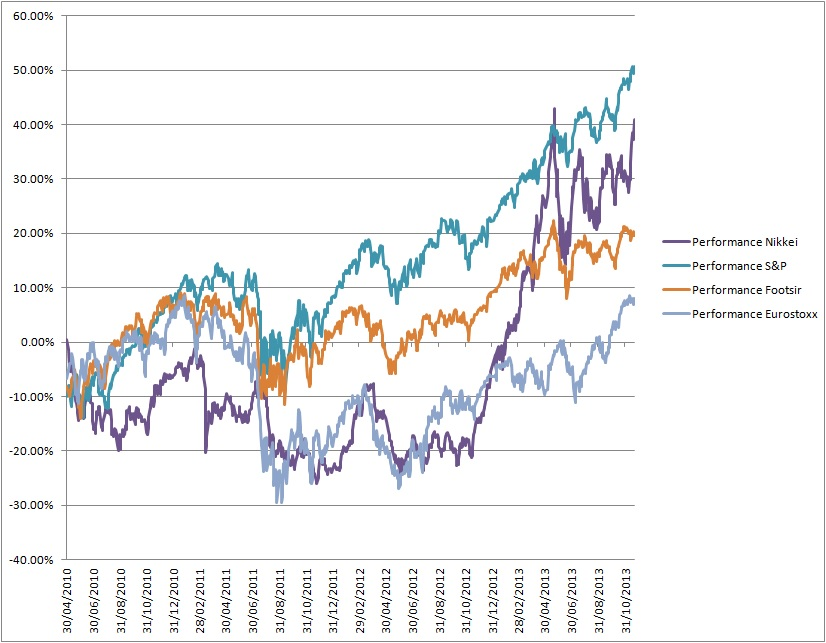
\includegraphics[scale=0.5]{Correlations_indices.jpg}
\end{center}

On constate suite à l'observation de ce graphique que l'évolution des performances du Footsie 100 et du S \& P 500 sont souvent dans les mêmes proportions et on observe les mêmes pics ainsi que les mêmes creux dans la plupart des cas comme par exemple au niveau du 30/06/2012.
Ceci offre donc de l'information à l'investisseur puisque celui-ci en anticipant une forte hausse du S \& P par exemple saura que le Footsie et le Nikkei toutes proportions gardées, devraient sentir une hausse sensiblement identique or comme les performances sont évalués sur 3 indices et que les meilleurs taux de rendements actuariels sont obtenus pour des échéances de un et deux ans. Ceci implique que l'investisseur pourra espérer obtenir le meilleur rendement actuariel possible avec ce produit.

\newpage



\section{Modèles Mathématiques}
Afin de proposer le produit Playlist aux clients, il faut en déterminer le prix. L'importance de la modélisation est donc capitale. En effet, nous devons faire des prévisions sur l'évolution des différents éléments financiers qui vont impacter sur le prix du produit. Le payoff du produit Playlist est directement lié à l'évolution des 4 indices présentés plus haut. Nous allons voir que pour modéliser l'évolution de ces indices, il nous faudra aussi modéliser l'évolution du taux sans risque, ainsi que la volatilité. Or il existe plusieurs modèles, plus ou moins raffinés, permettant de décrire la dynamique des actifs sous-jacents qui nous concernent et ces deux paramètres. Il convient donc de les présenter, et de faire un choix de modélisation.

\subsection{Modélisation des indices}

\subsubsection{Modèle de Black-Scholes}
Le modèle de Black et Scholes permet de modéliser le cours des actions. Mais il permet aussi de modéliser l'évolution des indices comme nous le verrons un peu plus loin. Il repose sur les hypothèses suivantes :
\begin{itemize}
\item[•] Absence d'Opportunité d'Arbitrage
\item[•] Absence de coûts de transaction
\item[•] Pas de restriction sur les ventes à découvert
\item[•] Le marché est continu
\item[•] Absence de dividendes
\item[•] Le taux sans risque \textbf{r} est constant quelle que soit la maturité
\end{itemize}
\\ \\
Dans le modèle de Black-Scholes, le cours du sous-jacent S vérifie l'équation stochastique :

$$ dS = \mu Sdt + \sigma SdW $$  \\
avec $W_{t}$ un processus de Wiener, $ W_{t} \rightarrow \mathcal{N}(0,\sqrt{t}) $ \\

On obtient avec Itô : \\
$$ d(ln(S))=(\mu - \frac{\sigma^{2}}{2})dt + \sigma dW $$ \\
Soit \\
$$ S(t) = S_{0} exp \left[(\mu - \frac{\sigma^{2}}{2})t + \sigma W \right] $$ \\

Le principal problème avec le modèle de Black-Scholes est qu'il ne présente pas une queue de distribution suffisamment lourde par rapport à la réalité : il ne prend pas en compte la possibilité de saut d'un cours boursier. Le modèle qui suit est le modèle de Merton. Celui-ci permet de prendre en compte cette possibilité.\\

\subsubsection{Modèle de Merton}
Le modèle de Merton introduit la possibilité de saut d'un cours boursier à l'aide d'un processus de Poisson :\\

$$ S(t) = S_{0} exp \left[(\mu - \frac{\sigma^{2}}{2})t + \sigma dW + \sum_{k=1}^{N(t)} U(k) \right] $$ \\
où
\begin{itemize}
\item[•] N est un processus de Poisson
\item[•] U est une suite de variables aléatoires iid suivant une loi normale centrée
\item[•] W, N et U sont des processus indépendants les uns des autres
\item[•] Les paramètres concernant U et N, ainsi que $\mu$ et $\sigma$ peuvent être estimés par la méthode du maximum de vraisemblance, entre autres
\end{itemize}
\\

\subsubsection{Modèle de Heston}
Les deux modèles précédant prennent pour hypothèse que la volatilité est constante. La réalité montre que celle-ci a une forme de smile, lorsque le prix d'exercice ou la maturité varie. Le modèle de Heston attribue donc à la volatilité une dynamique particulière : \\
$$ dV(t) = K(\theta - V(t))dt + \sigma \sqrt{V(t)} dW_{v}(t)  $$ \\
et \\
$$ \frac{dS(t)}{S(t)} = rdt + \sqrt{V(t)}dW_{s}(t) $$ \\
Où r est le taux sans risque, V la volatilité, K un paramètre de retour à la moyenne, $\theta$ la variance long terme, $\sigma$ la volatilité de la volatilité, et  $W_{s}$ et $W_{v}$ sont deux mouvements browniens corrélés.\\

\subsubsection{Choix du modèle et validité du modèle de Black-Scholes pour les indices}
Le modèle de Heston est reconnu comme étant le plus précis. Cependant, le nombre de paramètres étant très important, le calibrage de ces paramètres est très difficile à partir des ressources dont nous disposons. Le modèle de Black-Scholes étant le plus simple à implémenter, nous nous concentrerons tout d'abord sur celui-ci. L'implémentation du modèle de Merton pourrait représenter une bonne voie d'approfondissement, si le temps nous le permettait. \\ \\
Le modèle de Black-Scholes est le plus souvent utilisé pour modéliser la dynamique du cours d'une action boursière. Montrons qu'il peut aussi modéliser l'évolution d'un indice boursier. \\
Un indice peut être assimilé à un portefeuille d'actions. On note :
\begin{itemize}
\item[•] $P_t$ la valeur de l'indice à l'instant $t$, $t \in \mathbb{R}^{+} $
\item[•] $n$ le nombre d'actions qui composent l'indice
\item[•] $S_{i}(t)$ le cours de l'action $i$ à l'instant $t$, $t \in  \mathbb{R}^{+} $ et $i \in [[1,n]] $
\item[•] $ \omega_i (t) $ la proportion du titre $i$ dans l'indice, soit la capitalisation boursière de l'action i sur la capitalisation totale
\item[•] $N_i $ le nombre de titres respectifs, supposé constant au cours du temps\\
\end{itemize}
\\
On a donc à l'instant $t$ :
$$P_t = \sum_{i=1}^{n}N_{i}S_{i}(t) $$
On peut écrire pour chacune des actions l'égalité suivante :
$$ N_{i}S_{i}(t) = \omega_i(t)P_t $$
De plus, on considère un intervalle de temps infinitésimal $dt$. On a :
$$ P_{t+dt} = \sum_{i=1}^{n}N_i(S_i(t+dt) + d_{i,t}) $$
où $d_{i,t}$ sont les dividendes distribués par l'entreprise $i$ entre $t$ et $t+dt$. S'il n'y a pas de distribution de dividendes pendant cette période, alors $d_{i,k}=0$.
\\
\\
Le rendement instantané du portefeuille s'écrit :
$$ \frac{dP_t}{P_t} = \frac{P_{t+dt}-P_t}{P_t} = \sum_{i=1}^n\frac{N_i}{P_t}(S_i(t+dt)-S_i(t) + d_{k,t})   $$
Or, d'après la deuxième équation,
$$ \frac{N_i}{P_t} = \frac{\omega_i(t)}{S_i(t)} $$
Donc
$$ \frac{dP_t}{P_t} = \sum_{i=1}^n\frac{\omega_i(t)}{S_i(t)}(S_i(t+dt)-S_i(t) + d_{k,t}) $$
\\
On note $ dS_{i,t} = S_i(t+dt)-S_i(t)+d_{k,t} $. \\
On peut donc écrire
$$ \frac{dP_t}{P_t} = \sum_{i=1}^n\omega_i(t)\frac{dS_{i,t}}{S_i(t)} $$
\\
Notre hypothèse principale, est que chaque cours des différentes actions suit une dynamique de Black-Scholes. On a  :
$$ \frac{dS_{i,t}}{S_i(t)} = \mu_idt + \sigma_i dW_{i,t} $$  \\
avec $W_{i,t}$ un processus de Wiener, $ W_{i,t} \rightarrow \mathcal{N}(0,\sqrt{t})$.\\

Le rendement instantané du portefeuille est donc :
$$ \frac{dP_t}{P_t} = (\sum_{i=1}^n\omega_i(t)\mu_i)dt + \sum_{i=1}^n\omega_i(t)\sigma_idW_{i,t} $$ \\
On a $ dW_{i,t} \rightarrow \mathcal{N}(0,\sqrt{dt})$, donc on peut écrire $dW_{i,t} = U_i\sqrt{dt}$ avec $U_i \rightarrow \mathcal{N}(0,1)$ de loi centrée réduite. \\
On pose
$$\mu = \sum_{i=1}^n\omega_i(t)\mu_i$$ et $$V = \sum_{i=1}^n\omega_i(t)\sigma_iU_i$$

$V$ est une combinaison linéaire de variables aléatoires de loi normale centrée réduites. Elle suit donc une une loi normale centrée, mais non réduite. Elle peut donc s'écrire sous la forme $V = \sigma U$, où $U \rightarrow \mathcal{N}(0,1)$ et $\sigma^2$ est la variance de $Y$, et vaut :
$$\sigma^2 = \sum_{i=1}^n\sum_{j=1}^n\omega_i(t)\omega_j(t)\sigma_i\sigma_j\rho_{i,j} $$ \\
où $\rho_{i,j}$ est le coefficient de corrélation entre $U_i$ et $U_j$. \\\\
On peut donc écrire :
$$ \frac{dP_t}{P_t} = \mu dt + \sigma U \sqrt{dt} $$
En posant $dW = U \sqrt{dt}$, on a $dW \rightarrow \mathcal{N}(0,\sqrt{dt})$ est un processus de Wiener. \\ \\
On peut donc légitimement modéliser l'évolution de la valeur d'un indice boursier avec la méthode de Black-Scholes, en supposant que le cours de chacune des actions qui le composent suivent une dynamique de Black-Scholes.


\subsection{Modélisation de la volatilité}
L'un des paramètres les plus déterminants dans la modélisation des indices est la volatilité. Il faut donc être en mesure de modéliser cette volatilité afin de l'utiliser comme paramètre dans la modélisation des indices.\\ \\
Plusieurs modèles existent :
\begin{itemize}
\item[•] La volatilité \textbf{constante} : c'est le modèle le plus simple
\item[•] La volatilité \textbf{stochastique} : comme dans le cas du modèle de Heston, on attribue une dynamique particulière à la volatilité
\item[•] La volatilité \textbf{locale} : c'est un cas particulier de volatilité stochastique, où l'on considère que la volatilité dépend uniquement du cours de l'actif sous-jacent et du temps ($\sigma = f(S_{t},t)$)
\end{itemize}
\\
Étant donné que nous nous concentrons dans un premier temps sur l'implémentation du modèle de Black-Scholes, et que celui-ci suppose que la volatilité est constante, nous allons tout d'abord nous intéresser à celle-ci.  Les deux principaux estimateurs de ce paramètre sont la volatilité historique et la volatilité implicite.

\subsubsection{Volatilité historique}
Elle est mesurée par l'écart-type du rendement du sous-jacent, durant la période qui précède l'émission des options. En rapprochant les observations du cours du sous-jacent, on peut donc estimer la volatilité instantanée.\\

On peut donc considérer la racine carrée de la variance empirique sans biais comme son estimation :\\
$$ \widehat{\sigma^{2}} = \frac{1}{n-1} \sum_{i=1}^n (ln(\frac{S_{t}}{S_{t-1}}) - \widehat{\mu})^{2}    $$ \\
avec \\
$$ \widehat{\mu} = \frac{1}{n} \sum_{i=1}^n ln(\frac{S_{t}}{S_{t-1}})  $$ \\
où $n$ est le nombre d'observations, $S_{t}$ le cours du sous-jacent à l'instant $t$. \\ \\
Par convention, l'unité de temps pour mesurer les paramètres est l'année. Il faut donc annualiser la volatilité calculée, en supposant que le nombre de jours ouvrés est 252 jours : \\
$$ \sigma_{an} = \widehat{\sigma} \sqrt{\frac{252}{\Delta t}}  $$ \\
avec $\Delta t $ l'intervalle de temps entre deux observations consécutives.\\ \\
Concernant le nombre d'observations, d'après Hull, utiliser les données des cours les plus récents sur un durée de l'ordre de grandeur de la maturité du produit à modéliser. En effet, utiliser des observations trop éloignées va biaiser l'estimation, de même qu'avoir trop peu d'observations. Ici, il faudra donc se baser sur les données des six années précedant la mise sur le marché du produit Playlist.\\

\subsubsection{Volatilité implicite}
La volatilité implicite est obtenue à partir du prix de marché des options, en inversant l'équation :
$$ C_{BS}(\sigma) = C $$ \\
où $C_{BS}$ est le prix de l'option calculée avec la méthode de Black-Scholes, et $C$ est son prix observé sur le marché.\\

\subsubsection{Choix du modèle}
Etant donné que le calcul de la volatilité implicite nécessite d'avoir recours à des méthodes numériques pour inverser la formule (notamment la méthode itérative de Newton-Raphson) car celle-ci fait intervenir des intégrales, nous nous orienterons dans un premier temps vers le calcul présenté plus haut de la volatilité historique.

\subsection{Modélisation des taux d'intérêts}

Afin de pouvoir évaluer le produit structuré, nous devons aussi réussir à modéliser le taux sans risque. Plusieurs modèles de taux existent, présentant chacun des avantages et des inconvénients.\\
Le taux qui va nous intéresser est le taux sans risque zéro coupon de moyen-long terme comme il est question d'années avant l'échéance du produit Playlist. Il existe 3 catégories de modèles de taux : les modèles à 1 facteur, à 2 facteurs et ceux de type Heath-Jarrow-Morton (HJM).

\subsubsection{Modèles à un facteur}

Le \textbf{modèle de Vasicek} fait partie des premiers modèles de taux. Il repose sur l'hypothèse que les déformations de la structure du taux d'intérêt sont expliqués par le mouvement du taux court.\\
Le taux court suit une diffusion de type Ornstein-Uhlenbeck : \\
$$ dr_{t} = a(b-r_{t})dt + \sigma dW_{t} $$ \\
où
\begin{itemize}
\item[•] a est la force de rappel de retour à la moyenne
\item[•] b est le taux d'intérêt de long terme
\item[•] $\sigma$ est l'écart-type de variation instantanée de $r_{t}$ (volatilité instantanée)
\item[•] $dW_{t}$ est un mouvement brownien
\end{itemize}
\\

La remarque négative que l'on peut faire sur ce modèle est que la proportion de taux négatifs est parfois importante. Cela crée des distorsions fortes dans la valorisation de certains produits dérivés.\\ \\

Le \textbf{modèle de Cox-Ingersoll-Ross} est proche de celui de Vasicek, en présumant que le taux court suit la dynamique suivante :\\
$$ dr_{t} = a(b-r_{t})dt + \sigma \sqrt{r_{t}} dW_{t} $$
avec a, b, $\sigma$,et $dW_{t}$ similaires au modèle de Vasicek.\\
La principale remarque qu'on peut faire sur ce modèle est que le taux court n'est pas un processus gaussien, ce qui complexifie les calculs. \\ \\

Le \textbf{modèle de Black-Derman-Toy}  est un modèle log-normal :
$$ d(logr_{t}) = (b_{t} - a_{t} logr_{t})dt + \sigma dW_{t} $$

Le problème avec les modèles log-normaux est qu'on observe des proportions trop élevées de taux importants pour des horizons lointains, par rapport à la réalité.\\ \\

Le \textbf{modèle de Ho et Lee} est aussi utilisé pour modéliser l'évolution du taux court : \\
$$ dr_{t} = \theta_{t}dt + \sigma dW_{t} $$
avec $\theta_{t}$ la moyenne du taux court, évoluant dans le temps. \\
Ce modèle présente le même problème que celui de Vasicek dans le sens où l'on observe des taux négatifs. De plus, il ne prend pas en compte le phénomène de retour à la moyenne, à la différence des trois modèles précédents.\\ \\

Ces modèles ont la particularité d'être simples, cependant il est généralement reconnu que l'intégration d'une unique variable d'état ne permet pas de reproduire le comportement des courbes de taux observées. C'est pourquoi nous introduisons ici les modèles à 2 facteurs.


\subsubsection{Modèles à deux facteurs}
Le premier modèle bi-factoriel que nous allons présenter est le \textbf{modèle de Hull et White}. Ici on prend pour hypotèse que les coefficients varient en fonction du temps, et que les taux courts et taux longs suivent les deux dynamiques suivantes : \\
Taux court
$$ dr_{t} = K_{r}(l_{t} - r_{t})dt + \sigma_{r}dW_{r,t}  $$ \\
Taux long
$$ dl_{t} = K_{l}(\mu_{l} - l_{t})dt + \sigma_{l}dW_{l,t}  $$ \\
avec
\begin{itemize}
\item[•] $K_{r}$ et $K_{l}$ les vitesses de retour à la moyenne pour les taux courts et taux longs
\item[•] $\sigma_{r}$ et $\sigma_{l}$ leurs volatilités
\item[•] $\mu_{l}$ le taux long à 50 ans
\end{itemize}
\\
Les avantages de ce modèle est qu'il prend bien en compte le retour à la moyenne, et que sa discrétisation est exacte. Il faut tout de même préciser que les taux peuvent être négatifs, et que l'on n'observe pas la volatilité. \\ \\


Dans le \textbf{modèle de Fong et Vasicek} les deux variables d'état utilisées sont le taux court $r_{t}$ et la variance du taux court $\nu_{t}$ : \\
$$ dr_{t}=\alpha(b-r_{t})dt + \sqrt{\nu(t)}dW_{1}(t) $$
$$ d\nu_{t}=\gamma(c-\nu_{t})dt + \xi\sqrt{\nu(t)}dW_{2}(t) $$
avec
\begin{itemize}
\item[•] b et c les moyennes long terme du taux instantané et de sa variance
\item[•] $\alpha$ et $\gamma$ leurs vitesses de retour à la moyenne
\end{itemize}
\\
Ce modèle présente l'avantage de tenir compte du retour à la moyenne et de ne donner que des taux courts positifs.
Cependant, la complexité de la dynamique de la variance le rend difficilement exploitable.\\ \\


Le dernier modèle bi-factoriel que nous allons présenter est le \textbf{modèle de Lonstaff et Schwartz}. Les dynamiques des deux variables d'état sont des processus d'Ornstein-Uhlenbeck :
$$ dx_{t} = a(b-x_{t})dt + c\sqrt{x_{t}}dW_{2}(t) $$
$$ dy_{t} = a(e-y_{t})dt + f\sqrt{y_{t}}dW_{3}(t) $$ \\
Le taux instantané s'écrit au moyen de ces deux processus par : \\

$$ dr_{t} = (\mu x_{t} - \theta y_{t})dt + \sigma \sqrt{y_{t}}dW_{1}(t) $$ \\
où $W_{2}$ est non corrélé avec $W_{1}$ et $W_{3}$, et $\theta > \sigma^{2} $ assure la non-négativité de $r_{t}$.\\

Le principal problème de ce modèle est son nombre important de paramètres : 11 en tout.
 
\subsubsection{Modèles de Heath-Jarrow-Morton}
L'approche HJM est fondée sur la volonté de construire un modèle respectant la courbe des taux initiale, prise comme point de départ : on assimile le sous-jacent à l'entière courbe des taux dont la dynamique repose sur les taux forwards instantanés.

\subsubsection{Retrouver le taux zero-coupon}
La quasi-totalité des modèles que nous avons présenté permettent d'obtenir la dynamique du taux court $r_{t}$. Cependant, dans le cas de l'évaluation du produit structuré Playlist, il est important de déterminer les taux zéro coupon de moyen-long terme, car les échéances se comptent en années. On peut les obtenir de la manière suivante : \\

On suppose qu'on a la dynamique du taux court $r_{t}$. Le prix des zéro-coupon d'échéance T peut s'exprimer sous la forme \\
$$ P(t,T)=A(t,T)e^{-B(t,T)r_{t}} $$ \\
avec A et B qui diffèrent selon les modèles que l'on utilise. On sait de plus que \\
$$ P(t,T)= e^{-R(t,T)(T-t)}  $$ \\
avec R(t,T) le taux zéro-coupon d'échéance T. On peut récupérer R(t,T) en résolvant l'équation suivante : \\
$$ R(t,T)=-\frac{1}{T-t}ln(P(t,T)) $$ \\

\subsubsection{Choix du modèle}
Si les modèles HJM ou bi-factoriels permettent d'obtenir des courbes beaucoup plus précises de taux zéro-coupon, le modèle le plus abordable serait celui de Vasicek unifactoriel. Le modèle de Black-Scholes pour la simulation des indices nécessite un taux sans risque constant, c'est pourquoi nous commencerons par calculer à partir des données observées sur les marchés, un taux sans risque constant. Dans un deuxième temps seulement, nous essaierons d'implémenter et d'intégrer le modèle de Vasicek unifactoriel dans nos modélisations des indices.

\subsection{Modélisation des taux de changes}
Le produit Playlist fait intervenir des sous-jacents qui sont cotés en devise étrangère. La couverture sur ces produits est donc soumise à l'évolution des taux de changes.
Nos connaissances actuelles en la matière de nous permettent pas de choisir un modèle de taux de change sophistiqué. En revanche, nous savons que le modèle le plus simple, qui sera implémenté dans la première version, qui consiste à considérer le taux de change constant, n'apporte aucune valeur ajoutée à la modélisation. Nous nous bornerons donc dans un premier temps à l'approximation qui consiste à considérer que tous les sous-jacents sont exprimés en devise domestique.

\section{Analyse logicielle}

\subsection{Cahier des charges}
Il s'agit ici de faire l'inventaire des fonctionnalités indispensables que doit fournir notre application. Elles seront présentés par ordre d'importance, et détaillées en sous fonctionnalités si besoin est.
\\
\indent Dans un premier temps, le gestionnaire doit avoir la possibilité de consulter les informations globales concernant le produit. Ces informations comportent par exemple la date de début de validité du produit soit le 28 avril  2010 ainsi que la date actuelle ou bien la date d'échéance qui sera maintenant de façon certaine le ... avril 2016. Hormis ceci, le gestionnaire doit également pouvoir voir le nombre de parts acquises par les investisseurs ainsi que le nombre de parts disponibles au total et les valeurs que chacun de ces deux ensembles représentent en terme de cash. Toutes ces informations devront être réunies dans un même cadre (page web).\\
\indent \\
\indent Le gestionnaire doit également avoir la possibilité de voir l'évolution des différents indices, il doit ainsi avoir accès à la performance actuelle du fonds.

\indent \\
\indent Le gestionnaire doit avoir la possibilité de voir la composition de son portefeuille et notamment la répartition en pourcentage ou bien en quantité de chacun de ces investissements. Il pourra ainsi avoir la valeur liquidative de chacune de ses parts. Le gestionnaire doit également avoir la possibilité de choisir le modèle d'évolution des sous jacents, que ce soit Black-Scholes ou bien le modèle de Merton, qu'il souhaite utilisé pour évaluer cette valeur. 
\indent \\
\indent Aussi, le gestionnaire doit avoir accès à un proposition de couverture, dans le cadre du modèle choisit. Plus précisément le gestionnaire ne devra pas avoir la possibilité de modifier le modèle en cours de simulation par soucis de cohérence. De plus le gestionnaire devra avoir la possibilité d'indiquer ses propres dates de rebalancement.\\
On laissera la possibilité au gestionnaire de se couvrir différemment de ce qui est préconisé, ce qui implique que celui-ci aura la possibilité de relancer une simulation à partir de la composition de portefeuille qu'il a choisi. Il pourra donc entrer la composition de son nouveau portefeuille.\\
\indent \\
\indent Enfin, il aura également la possibilité d'accéder à une simulation des cours futurs et de l'erreur commise à maturité pour une trajectoire particulière en supposant qu'il ai suivit aujourd'hui, et chaque fois qu'elles lui auront été proposées, les recommendations de rebalancement. Il s'agit de le convaincre du bien fondé de ces propositions.

\subsection{Architecture logiciel globale}

Voici une première schématisation de l'architecture de notre produit.

\begin{center}
\caption{Architecture}
\end{center}

\begin{center}
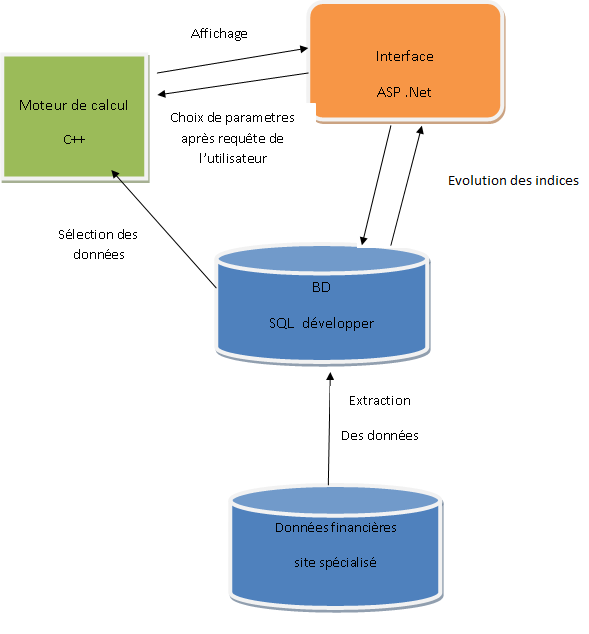
\includegraphics[scale=0.5]{graphe.png}
\end{center}

\noindent Ainsi on constate que l'architecture que nous avons adopté se base sur les cours disponibles sur des sites spécialisés tels que \lstinline!yahoo finance!, ainsi à partir d'un extracteur de données, nous récupérerons les données de ce site concernant les indices voulus, ce qui alimentera notre base de données. Les données seront alors traitées par le moteur de calcul notamment pour connaître la performance actuelle du fonds, avoir diverses modélisations de l'évolution des indices. Il vient alors l'interface qui à l'aide des sorties du moteur de calcul peut afficher l'évolution des différents indices ainsi que la performance du fonds.\\
On constate également la présence d'un lien entre l'interface et la base de données en effet, lorsque l'utilisateur sélectionne de nouvelles dates pour voir l'évolution des différents indices, il n'est pas nécessaire de faire appel au moteur de calcul.

Si l'on rentre un peu plus dans le détails, on peut modéliser l'architecture de la façon suivante :


\begin{center}
\caption{Architecture globale}
\end{center}

\begin{center}
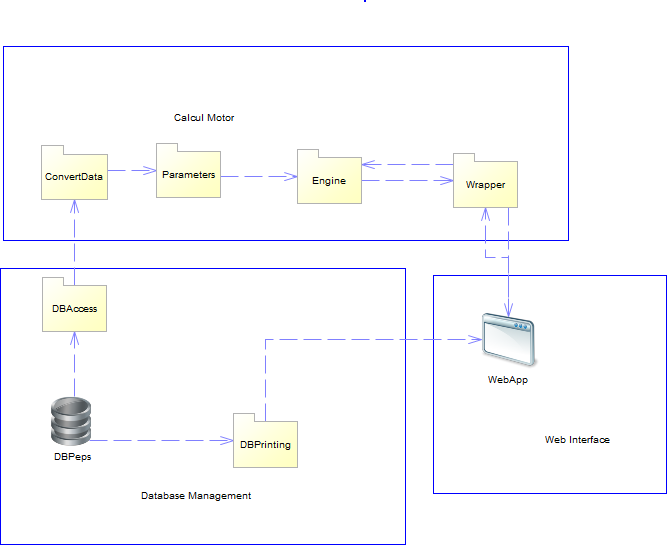
\includegraphics[scale=0.8]{GloabalDiag.png}
\end{center}

On constate dans cette architecture que l'intégralité de la partie calcul s'effectuera en C++ grâce à l'utilisation de deux modules C++/CLI. C'est pourquoi, on aura deux packages de traitement de la base de données, en effet le premier \lstinline!DBPrinting! sera directement relié à l'application web pour afficher notamment le cours actuel des indices. L'autre \lstinline!DBAccess! permettra de transmettre le nécessaire au calcul des paramètres et donc au calibrage de notre modèle. Les différents paramètres étant calculés, \lstinline!Engine! interviendra pour réaliser les différentes simulations, et donc calculer le prix ainsi que le vecteur associé à la couverture ainsi que le P\&L. Les relations sont dans les deux sens entre \lstinline!WebApp! et le \lstinline!Wrapper! ainsi que entre le \lstinline!Wrapper! et \lstinline!Engine! car comme précisé précédemment le gestionnaire à par exemple la possibilité de donner la composition de son portefeuille, les informations relatives doivent donc redescendre jusqu'à \lstinline!Engine! pour que cela soit pris en compte.

\subsection{Architecture détaillée}

De façon plus précise, l'architecture précédente peut être explicité comme suit :

\newpage

\begin{landscape}
\begin{figure}[h!]
  \caption{Architecture détaillée.}
  \centering
    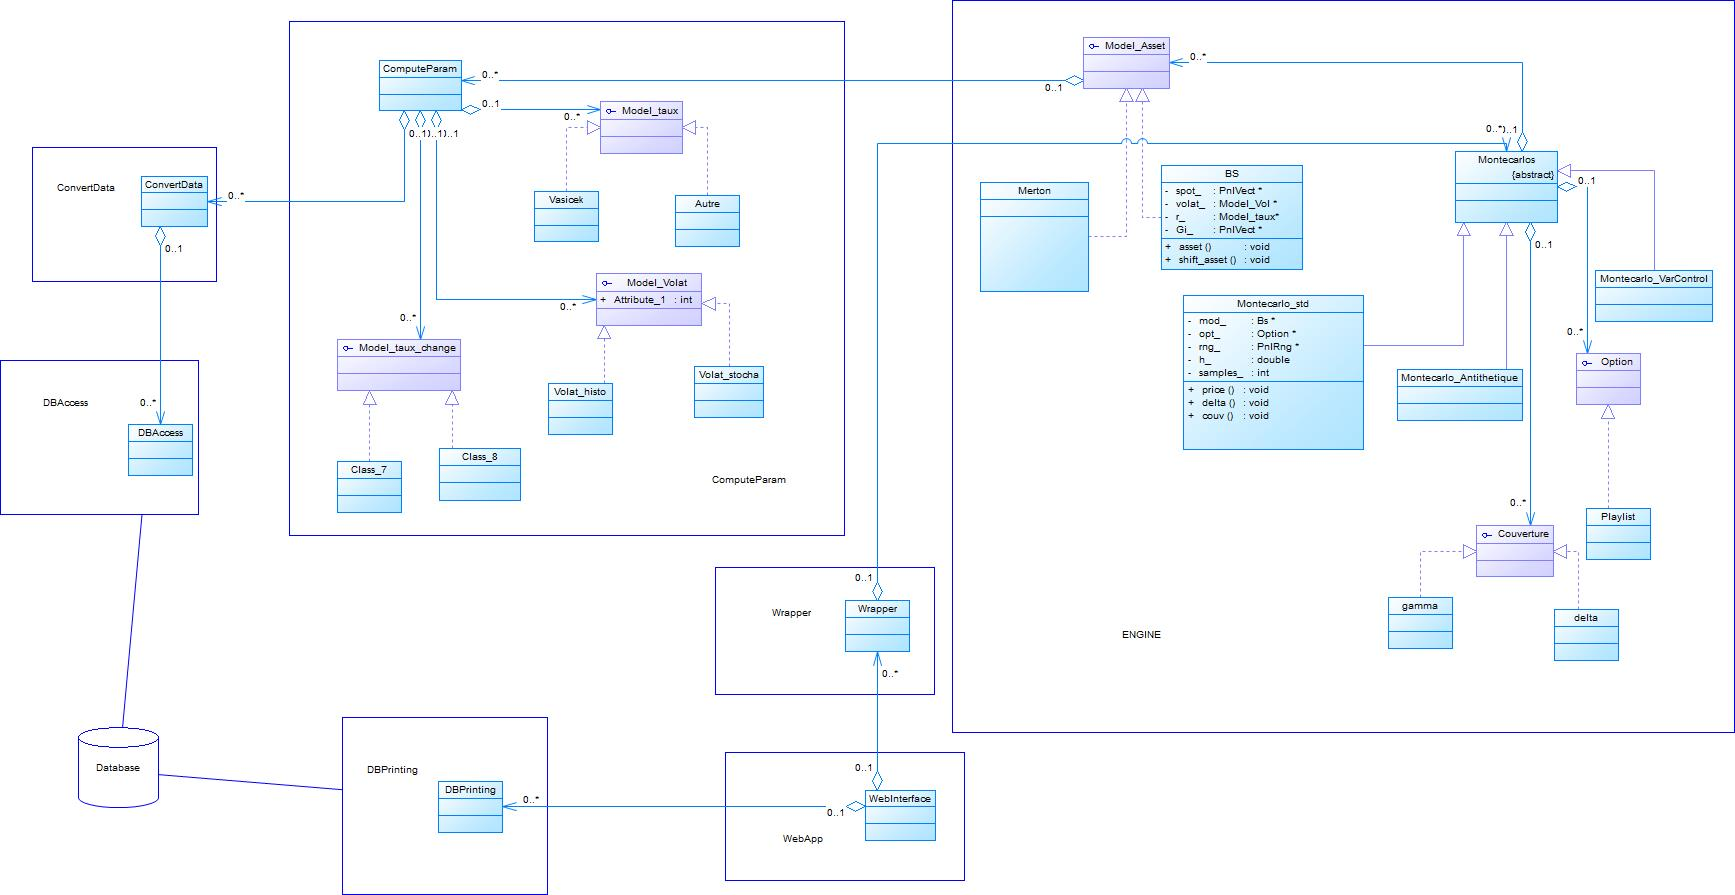
\includegraphics[height=14cm, width = 20cm]{DiagClasse.jpg}
\end{figure}
\end{landscape}

On peut ainsi voir dans cette structure les différents packages présentés précédemment, nous avons de plus choisi d'utiliser de nombreuses classes abstraites, l'objectif étant de modéliser par exemple les différents modèles de taux que le gestionnaire peut choisir, les différentes évolutions du sous-jacents ou bien encore le type d'évolution de la volatilité. De plus par soucis d'efficacité et de cohérence, nous avons choisi de réaliser l'intégralité des calculs en C++, que ce soit pour obtenir les valeurs de la volatilité ou bien calculer le vecteur de couverture. De plus nous ne passons pas par cette voie pour afficher directement des données extraites de la base de données, dans ce cas particulier, la classe C\# \lstinline!DBPrinting! communiquera directement avec l'interface. La base de données associées sera la suivante :

\begin{figure}[h!]
  \caption{Base de données}
  \centering
    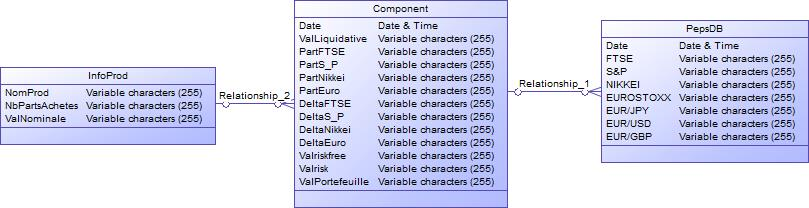
\includegraphics[scale=1]{BD.jpg}
\end{figure}

La base de données ne sera en effet pas plus compliquée puisque nous aurons besoin du cours des indices à tout moment ainsi que sotcker les différentes valeurs liquidatives et compositions de la couverture. Les deux tables précédentes sont donc suffisantes.

%\begin{center}
%\caption{Architecture Détaillée}
%\end{center}
%\begin{landscape}
%\begin{center}
%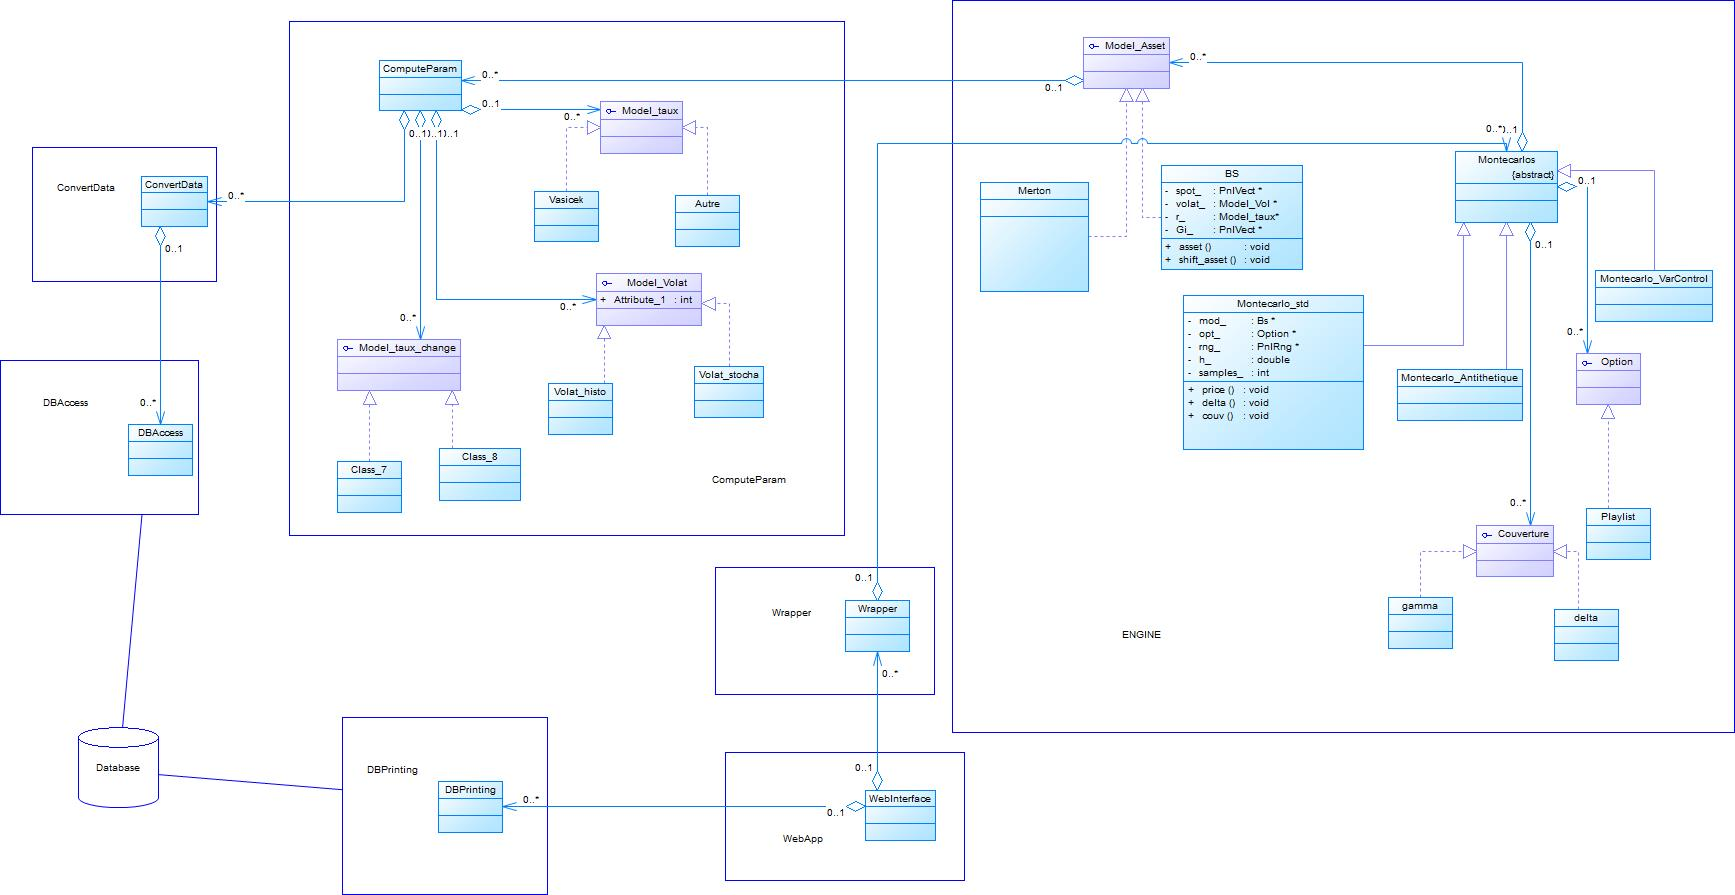
\includegraphics[scale=0.4]{DiagClasse.jpg}
%\end{center}
%\end{landscape}


\subsection{Spécifications}

Nous allons dans un premier temps expliciter ce qui se cache derrière la fonctionnalité couverture énuméré dans le cahier des charges.\\
La question de la couverture pose différents problèmes, en effet dans un premier temps nous réaliserons une couverture en delta. Ainsi pour une action devant répliquer les flux du fond que nous vendrons, nous cherchons à savoir quelle est la quantité de chaque indices que nous devons acheter pour s'assurer éviter des pertes et plus particulièrement supprimer le risque associé à l'option.\\
Ainsi dans un premier temps, il nous faut pricer l'option que nous proposons. Cela implique  de devoir fixer le modèle que nous allons utiliser pour modéliser l'évolution des sous jacents. Ainsi nous avons choisi dans un premier temps d'implémenter le modèle de Black& Scholes. Se pose alors la question des différents paramètres du modèle, nous avons dans un premier temps choisi de déterminer la variance à l'aide d'un backtest sur les valeurs des différents indices au cours des trois derniers mois, nous ferons de mêmes pour déterminer la matrice des corrélations. En ce qui concerne les autres paramètres tels que le taux sans risque ou bien la probabilité historique, nous prendrons des valeurs arbitraire en essayant de coller au maximum avec les valeurs dont nous disposons.\\
Disposant alors d'un modèle, il nous faut définir les paramètres caractérisant notre option, aux vues des propriétés de celle ci énoncé précedemment, on lui attribuera une maturité fixée par défaut à 6, un nombre de date de constatation ainsi que la taille du modèle.
Enfin on considère un modèle de MonteCarlo pour obtenir le prix de notre option.\\
Par la suite, nous considérerons des modèles plus compliqués, c'est pourquoi nous avons choisi d'implémenter des classes abstraites pour que différents modèles puissent être ajouté.
C'est ainsi que nous obtenons le diagramme de classe suivant :\\  

\begin{center}
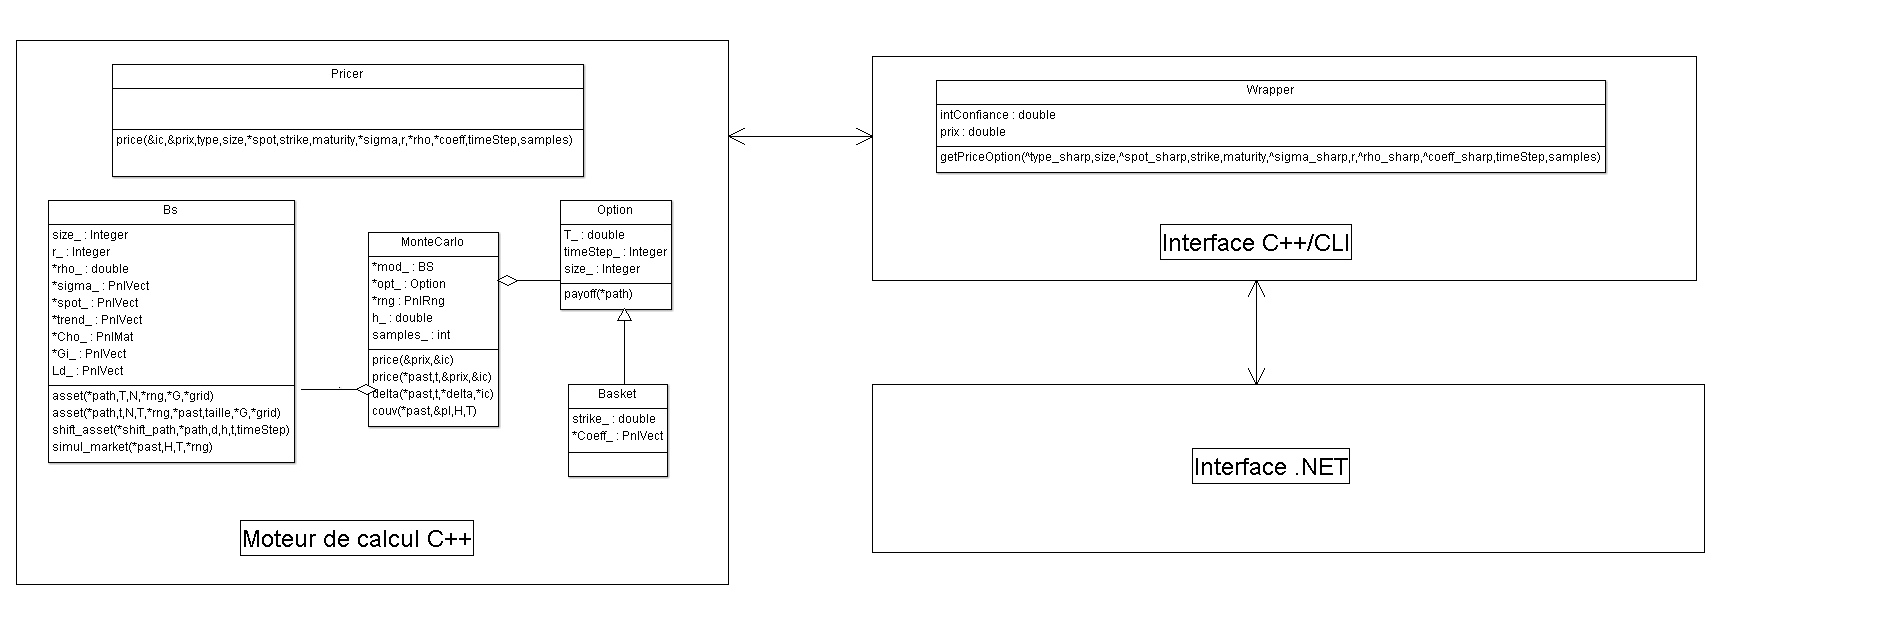
\includegraphics[scale=0.3]{class_diag.png}
\end{center}
 
 Un interface alors envisageable pour représenter les éléments décris précédemment pourrait être l'interface suivante :\\

\begin{center}
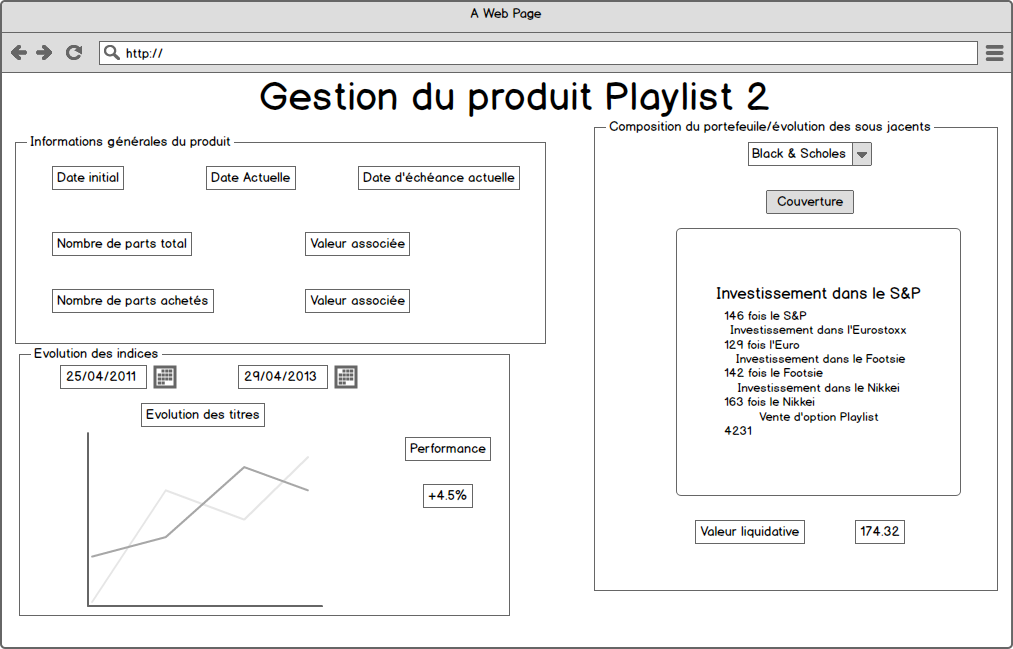
\includegraphics[scale=0.3]{maquette.png}
\end{center}

On fait ainsi apparaître dans l'onglet en haut à gauche, la date à laquelle à été prise la valeur liquidative de référence, la date actuelle ainsi que la date d'échéance prévu pour avoir une vision global de la chronologie du produit.\\
Nous faisons de plus apparaître le nombre de parts disponible à la base ainsi que le nombre de parts qui ont été acquise ainsi que les valeurs monétaires associées. Ceci permet de voir le taux d'acceptation du produit par le marché.\\
Le bloc situé en bas à droite permettra plutôt de voir l'évolution de la performance du produit ainsi on peut choisir la date de début ainsi que la date de fin, ce qui va nous permettre de visualiser l'évolution des différents indices concernés sur cette plage. Juste à côté nous afficherons la performance du fond sur cette plage.\\
Enfin le dernier bloc nous permet de choisir le modèle d'évolution des sous-jacents ce qui aura pour conséquence de modifier l'évolution des sous-jacents et ainsi la couverture proposée juste en dessous.
La couverture sera décrite par le nombre d'action vendue, correspondant aux nombres de parts vendues et le nombre de fois que l'on doit acheté chacun des indices. On en déduiera ainsi la valeur liquidative en dessous.

\section{Annexes}

\subsection{Pseudo code pour la valeur du flux versé en t}

\begin{verbatim}

flux(var ValNom, var temps){
   var flux = 0;
   var performance =0 ;
   var CountSupDix = 0;
   var CountSupVingtEnUn=0;
   var CountSupVingtEnDeux=0;
   var CountSupVingtEnMin=0;
   var borne = minimum(t,2);
   var verse = 0;
   Simulation des Indices
   Si le temps vaut 1 ou 2 ou 6
      Si le temps vaut 6
         Pour tout les indices parmi la Liste des Indices
            Si la performance de l'indice en 1 est supérieur à 20%
               on incrémente CountSupVingtEnUn de 1
            Fin SI
            Si la performance de l'indice en 2 est supérieur à 20%
               on incrémente CountSupVingtEnDeux de 1
            Fin SI
         Fin pour tout
         Si (CountSupVingtEnUn est inférieur à 3 et CountSupVingtEnDeux est inférieur à 3 )
            Verse passe à 1
         Fin SI
      Sinon si
         Pour tout les indices parmi la Liste des Indices
            Si la performance de l'indice en borne est supérieur à 20%
               on incrémente CountSupVingtEnMin de 1 
            Fin si
         Fin pour tout
         Si CountSupVingtEnMin est supérieur à 2
            verse passe à 1
         Fin si
      Fin si
   Fin si
   Si verse vaut 1
      Pour tout k entre 1 et t
         Pour tout les indices dans la Liste des Indices
            Si la performance de l'Indice en k est supérieur à 10%
               on incrémente CountSupDix de 1
            Fin si
         Fin pour tout
         Si CountSupDix est supérieur à 2
            on augmente la performance de 4.5%
         Fin si
      Fin pour tout
      On renvoie ValNom*(1+performance);
   Fin si
   On renvoie 0;
}
\end{verbatim}


\end{document}

